\setcounter{figure}{0}

\section{23rd July 2023: God in the midst of an angry man}
\subsection*{Text: Jonah 4}
  \begin{quote}
    [1] But it displeased Jonah exceedingly, and he was angry. [2] And he prayed to the LORD and said, “O LORD, is not this what I said when I was yet in my country? That is why I made haste to flee to Tarshish; for I knew that you are a gracious God and merciful, slow to anger and abounding in steadfast love, and relenting from disaster. [3] Therefore now, O LORD, please take my life from me, for it is better for me to die than to live.” [4] And the LORD said, “Do you do well to be angry?”

    [5] Jonah went out of the city and sat to the east of the city and made a booth for himself there. He sat under it in the shade, till he should see what would become of the city. [6] Now the LORD God appointed a plant and made it come up over Jonah, that it might be a shade over his head, to save him from his discomfort. So Jonah was exceedingly glad because of the plant. [7] But when dawn came up the next day, God appointed a worm that attacked the plant, so that it withered. [8] When the sun rose, God appointed a scorching east wind, and the sun beat down on the head of Jonah so that he was faint. And he asked that he might die and said, “It is better for me to die than to live.” [9] But God said to Jonah, “Do you do well to be angry for the plant?” And he said, “Yes, I do well to be angry, angry enough to die.” [10] And the LORD said, “You pity the plant, for which you did not labor, nor did you make it grow, which came into being in a night and perished in a night. [11] And should not I pity Nineveh, that great city, in which there are more than 120,000 persons who do not know their right hand from their left, and also much cattle?”
  \end{quote}
\subsection*{Notes}
\begin{itemize}
  \item{Last Sunday (Jonah 3), we learnt about God being a God of second chances.}
  \item{But here, we see Jonah being angry with God for being gracious. Jonah was upset with God’s character for being gracious, for being Himself.}
  \item{Unlike Jonah, the Ninevites did not know that God was gracious. Jonah knew that God would forgive the Ninevites if they repent. This is why he didnt want to go to Tarschich in general. He didnt want the Ninevites to enjoy God’s grace and mercy. As someone who has experienced God’s mercy himself (c.f chapter 2), it is quite selfish for Jonah to want to prevent others from experiencing God’s grace. Furthermore, who is Jonah to tell God who He can or cannot forgive?}
  \item{Knowing the truth about God should change our \textbf{posture} towards God. Jonah knew the truth about God’s character, but Jonah’s heart wasn’t changed. Especially in this context, we should be rejoice with other people and share their blessings with them. In the ideal situation, we should be able to rejoice even with our enemies when they do well.}
  \item{God’s response to Jonah was quite patient. Instead of chiding Jonah, He asked Jonah: “do you do well to be angry?” But Jonah didn’t reply God. Jonah just went into the desert to sulk. He was throwing an tantrum, he was showing God his displeasure at Him forgiving Nineveh.}
  \item{We also see how, despite Jonah’s disobedience, God appointed a plant to come up over Jonah, to shelter Jonah from the sun. Then Jonah was exceedingly glad because of the plant. But then, when God appointed a worm to eat the plant, and then when the plant died, Jonah became angry at God, angry enough to die.}
  \item{Through the plant, God is teaching Jonah a lesson. Jonah thinks that he is better than God, in the area of justice and in the area of compassion.
  \begin{itemize}
    \item{Jonah thinks he is more just than God because he thinks that it is unjust for God to forgive the Ninevites. How can God just let the Ninevites go scot free after they repent?}
    \item{Jonah thinks he is more compassionate than God because he cares about the plant more than God cares about the plant. How can God kill the plant prematurely?}
  \end{itemize}
  Here, we see the irony; Jonah cares more about the death of a plant than
  the death of 120000 people, as well as the cattle. }
  \item{The fundamental thing that Jonah forgot is this: there is none righteous, no, not one. Israel is not less sinful than Nineveh, and Jonah is not less sinful than Nineveh. It is only of God’s grace that in the OT, Israel is chosen by God to be His people. Everything is all of grace, and every person, jew or greek, professing christian or non Christian, are equally sinful and are in need of God’s grace.  }
  \item{In the parable of the prodigal son, the older brother is so resentful because he feels that he worked very hard but the father did not bless him. But from his tone, we know that the older brother’s service to his father is not joyful service, but is a burden. So the older son feels like he deserves better because of his hard work, as compared to the younger son who just repents. Two problems here:
  \begin{itemize}
    \item{The older brother’s POV is legalism. He thinks his works can earn his father’s favour.}
    \item{But more fundamentally, he doesn’t need to earn his father’s favour, because as the father said, “all that I have is yours”.}
  \end{itemize}}
  \item{We don’t need to work to earn our Father’s favour, we already have
  every spiritual blessing in the highest places. Hence, 
  \begin{itemize}
    \item{ Direct application: We should not feel resentful when we see other
    people who we think are “unworthy of God’s grace” come to God, because we
    are all unworthy. The older brother did not do anything to be born into
    his father’s family, so similarly, we did not do anything to be accepted
    by God as His children.}
    \item{Indirect application: We should not feel resentful or envious of other people when they seem to experience more physical blessings. We should not think: “God i serve in church every week, why am i still struggling financially but person X (which could be Christian) never do anything but still doing so well”. We must already know that we already have every spiritual blessing in the highest places.}
  \end{itemize}}

  % \item{\begin{figure}[H]
  %   \centering
  %   % 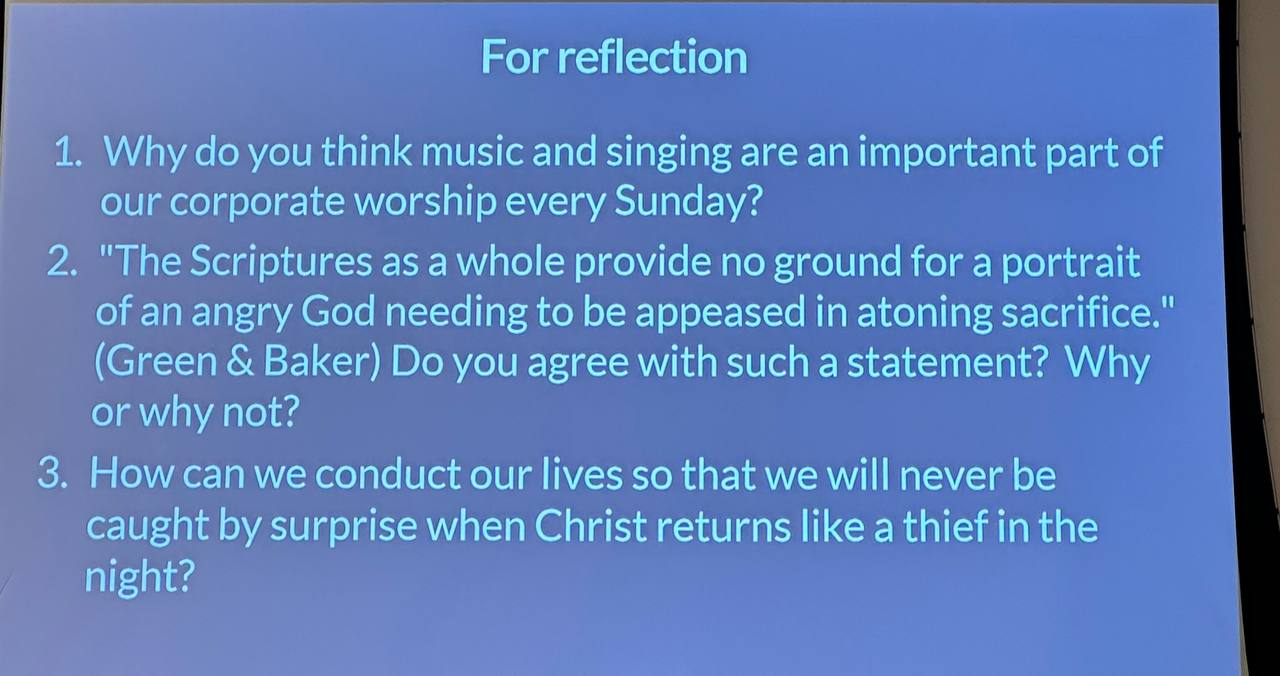
\includegraphics[width=0.8\textwidth, trim={0cm 0cm 0cm 0cm},clip]{Figures/marchSermon4Reflections.jpg}
  %   \includegraphics[width=0.8\textwidth, trim={0cm 0cm 0cm 0cm},clip]{example-image-a}
  %   \caption[]{Reflection questions for this sermon}
  %   \label{}
  % \end{figure}}
\end{itemize}